% =====================================================================
%  Lab 4: Spectroscopy -- ASTR UN1903, Fall 2026 (Noor, Thursday section)
%
%  ADAPTED FROM: "Lab 3: Spectroscopy" by Porter, Fall 2024 (Wed 6-9pm).
%  All explanatory text and figures are Porter's. Change history:
%   v1 -- questions rewritten as fill-in-on-the-sheet (circle/checkbox/blank).
%   v2 -- cut the CMB / Wien's-law-repeat question.
%   v3 -- REORDERED: lamp activity opens the lab, ahead of blackbody/PhET/
%         Wien's law. Star-vs-galaxy comparison moved with it. "Wrapping
%         things up" replaced with a short open reflection.
%   v4 -- PROMPT SHEET ONLY. Students answer in lab notebooks and submit
%         digitally, so all blanks, ruled lines, answer boxes and checkboxes
%         removed; choices printed as lettered options instead.
%   v5 -- Removed the "How to answer" instruction box from page 1 (cover it
%         verbally / on Courseworks). Removed all section time estimates.
%         Converted most multiple-choice and fill-in-the-blank items to
%         direct short-answer questions. MCQ retained ONLY where the
%         distractors do teaching work -- Q3 (element vs. temperature vs.
%         brightness) and Q19 (the photosphere/corona mechanism) -- since in
%         both cases the wrong answers are the misconceptions worth
%         surfacing. Answers stay short by asking for a word, a number, or
%         one sentence. Numbering UNCHANGED from v3/v4 (1-25).
% =====================================================================

\documentclass[11pt]{article}
\usepackage[includeheadfoot, top=1.0in, bottom=1.0in, hmargin=1.0in]{geometry}
\usepackage[utf8]{inputenc}
\usepackage{fancyhdr}
\usepackage{url}
\pagestyle{fancy}
\usepackage{setspace}
\usepackage{tabularx}
\usepackage{graphicx}
\usepackage{caption}
\usepackage{subcaption}
\usepackage{hyperref}
\usepackage{multicol}
\usepackage{amssymb}
\usepackage{enumitem}
\usepackage{array}

\lhead{Astronomy Lab I}
\rhead{Fall 2026}
\cfoot{\thepage}

% --- helpers ---------------------------------------------------------
% lettered answer options, used sparingly (Q3 and Q19 only)
\newenvironment{choices}
  {\begin{list}{}{%
     \setlength{\leftmargin}{2em}\setlength{\itemsep}{2pt}%
     \setlength{\topsep}{4pt}\setlength{\parsep}{0pt}}}
  {\end{list}}
\newcommand{\ch}[1]{\item[\textbf{(#1)}]}

% a reference wavelength scale, for students to copy when sketching
\newcommand{\wlscale}{\hbox to \linewidth{\footnotesize
  400\hfill 450\hfill 500\hfill 550\hfill 600\hfill 650\hfill 700\,nm}}
\newcommand{\scaleref}{%
  \par\smallskip\noindent
  \fbox{\parbox[b][1.1cm][b]{0.96\textwidth}{\wlscale}}\par\smallskip}

\setlist[enumerate]{itemsep=11pt, topsep=6pt}

\begin{document}

\begin{center}
\huge{Lab 4: Spectroscopy}
\end{center}

\medskip

%%%%%%%%%%%%%%%%%%%%%%% INTRO %%%%%%%%%%%%%%%%%%%%%%%
\section{Introduction: The Rainbow Connection}

\textbf{\emph{Spectroscopy}} is the study of the light that objects emit or absorb. Last lab, we saw that the Universe is filled with a myriad flavors of light, spanning orders of magnitude in wavelength. Spectroscopy hones in on a specific object and holistically studies the range of wavelengths emitted or absorbed by that object -- the set of light emitted or absorbed by an object is called the object's \textbf{\emph{spectrum}}. An object's spectrum can provide a remarkable amount of information; the spectrum tells us about the chemical makeup of the object, the motion and speed of the object, the temperature of the object, the distance to the object (in certain contexts), and much more. Thus, spectroscopy is an extremely popular technique for studying planets, stars, and galaxies. Much of what we know about these objects is \emph{because} of spectroscopy.

%%%%%%%%%%%%%%%%%%%%%%% LAMPS %%%%%%%%%%%%%%%%%%%%%%%
\section{Looking at Light}

Let's look at some lamps (or, diffusion tubes)! If you do not already have a \emph{diffraction grating} or \emph{spectroscope}, come get one from me. \textbf{Keep track of your diffraction grating/spectroscope and ensure it is returned at the end of the lab.} A diffraction grating splits light into its component colors, much like a prism. There are several lamps set up in the room; each lamp is actually heated gas of a specific element. Go up to each lamp and look at it through your diffraction grating. \textbf{Please do not touch the lamps, they are hot!} \\

Refer to the "Spectra\_Handout" PDF for help identifying the elements from their spectra.



\begin{enumerate}
    \item \textit{[9 points]} Sketch each lamp's spectrum in your notebook. Do all three
    lamps. For each one, write down the element and draw what you see.

    \smallskip
      Draw a horizontal strip for each lamp then mark roughly where the vertical lines fall. No need to color the lines, but try to describe the colors
    (``bright green,'' ``two close reds''). 

    \scaleref

    \item \textit{[2 points]} Note the similarities and differences in these spectra.

    \item \textit{[1 point]} Why do the lamps look different from each other through the grating? Choose an option from below.
    \begin{choices}
      \ch{a} Each lamp holds a different element, and each element emits its own
             set of wavelengths.
      \ch{b} Each lamp is a different temperature.
      \ch{c} Each lamp is a different brightness.
    \end{choices}

    \item \textit{[2 points]} Now look at one of the light bulbs (a source of white light) in the room through your diffraction grating. Describe what you see. How is the light bulb's spectrum different from
    the lamps?
\end{enumerate}

%%%%%%%%%%%%%%%%%%%%%%% BLACKBODY %%%%%%%%%%%%%%%%%%%%%%%
\section{Blackbody Radiation}

The light bulb gave you an unbroken rainbow. Where does that rainbow come from, and what decides which color is brightest in it? To answer that, we'll consider the simplified, idealized model of a \textbf{\emph{blackbody}}. A blackbody is an object that perfectly \emph{absorbs} all wavelengths of light, with no reflection. In addition to absorbing all wavelengths of light, a perfect blackbody will also \emph{emit} light at all wavelengths.

\begin{enumerate}
    \setcounter{enumi}{4}
    \item \textit{[3 points]} Consider the processes of \emph{emission}, \emph{absorption}, and \emph{reflection} (or \emph{``scattering''}) of light.
    Define each one in your own words. A short phrase each is plenty
        --- think about what happens to a beam of light when it meets an object.
        
\end{enumerate}

%The Planck Spectrum and Wien's Law
If one plots the intensity (or brightness) of light at each wavelength emitted by a blackbody, it yields the \emph{blackbody spectrum}. Blackbody spectra are smooth - we will soon find out that stars and other astronomical objects are not, but we can usually approximate them as blackbodies! 

For now, though, let's examine the blackbody spectrum hands-on. Navigate to \url{https://phet.colorado.edu/sims/html/blackbody-spectrum/latest/blackbody-spectrum_en.html}. The plot to the left of the screen shows a blackbody spectrum, with spectral power density (the amount of light emitted) on the vertical axis and wavelength on the horizontal axis; don't worry too much about these units. Make sure to check the boxes for ``Graph Values" and ``Labels" in the box to the upper right; after turning on these features, you should see a pair of yellow numbers labeling the \emph{peak} of the blackbody curve.

To the right of the screen is a thermometer showing the temperature of the blackbody. You can click and drag the slider on the thermometer to change the temperature of the object. If you need to adjust the size of your graph to see the full curve, you can use the zoom buttons (the magnifying glasses) to the upper left and bottom right of the plot.

\begin{enumerate}
    \setcounter{enumi}{5}

    \item \textit{[3 points]}  \textbf{Make a table in your notebook} with four columns:

    \smallskip
    \begin{center}
    \begin{tabular}{@{}llll@{}}
    \textbf{Temperature, $T$} & \textbf{Peak wavelength, $\lambda_{\rm peak}$} &
    $\mathbf{1/\lambda_{\rm peak}}$ & $\mathbf{\lambda_{\rm peak} \times T}$ \\
    (K) & ($\rm \mu m$) & ($\rm 1/\mu m$) & ($\rm \mu m\,K$)
    \end{tabular}
    \end{center}

    \smallskip
    Test \textbf{at least 5} different temperatures spread across the full range
    of the thermometer, and fill in the first three columns. Three of your five rows
    should be for the ones marked on the thermometer itself: the \textbf{light
    bulb}, \textbf{the Sun}, and \textbf{Sirius A}. Use
    \emph{two} significant figures. \textbf{Leave the last column empty for
    now.}

    \item \textit{[2 points]}  Look at your first two columns. As temperature goes \emph{up}, what
    happens to the peak wavelength? What is this type of relationship called?

    \item \textit{[3 points]}  Plot your data: $1/\lambda_{\rm peak}$ on
    the vertical axis, temperature on the horizontal axis. \textbf{Label both
    axes with the appropriate units.} What shape do your points make?

    \item \textit{[2 points]}  Now fill in the last column of your table ($\lambda_{\rm peak} \times
    T$, two sig figs). What do you notice about those five values?
\end{enumerate}

\medskip \noindent
Congratulations! You've just derived a key equation in astronomy, \textbf{Wien's law}. Because the product of the peak wavelength and the temperature is always the same number, we can determine the surface temperature of an object (like a star) by measuring the wavelength at which the object emits most of its light. In math, Wien's law reads
\begin{equation}
    \lambda_{\rm peak} \times T = \left(2.9 \times 10^3 \right) \, {\rm \mu m \, K},
\end{equation}
where $\lambda_{\rm peak}$ is the peak wavelength (in $\rm \mu m$) and $T$ is the temperature (in K). Let's use Wien's law to answer a few questions.

\begin{enumerate}
    \setcounter{enumi}{9}

    \item \textit{[1 point]} Are redder objects hotter or cooler than bluer objects? (this applies to both the flames on our kitchen stoves and to the stars illuminating the night sky).

    \item The surface temperature of the Sun is around $5780 \, {\rm K}$. 
    \begin{enumerate}
        \item \textit{[2 points]}  At which wavelength does the Sun emit most of its light (give your answer in $\rm \mu m$ to two sig figs)? Show your work.
        \item \textit{[1 point]} What color of light does the Sun emit the most? (Note: you can use the tool from the previous section).
    \end{enumerate} 
\end{enumerate}

%%%%%%%%%%%%%%%%%%%%%%% ELEMENTS %%%%%%%%%%%%%%%%%%%%%%%
\section{Fingerprints of the Elements}

The blackbody spectrum is a perfectly smooth spectrum --- like the light bulb. In reality, however, objects (like stars and galaxies) possess many ``features'' -- or \emph{lines} -- in their spectra, like the ones you sketched from the lamps, that can tell us much more than just the temperature of the object. Let's explore some real spectra now.

Figure \ref{fig:spec} shows examples of two different real spectra. On the horizontal axis, we have the wavelength of light (as was also the case in the blackbody spectrum); in general, spectra can cover wavelengths of light spanning the entire electromagnetic spectrum. On the vertical axis, we have \textit{flux}, another measure for how much light is being emitted and detected (in particular, flux measures the amount of light passing through a given area in a given amount of time).

\begin{figure}[h!]
    \centering
    \begin{subfigure}[b]{0.75\textwidth}
        \centering
        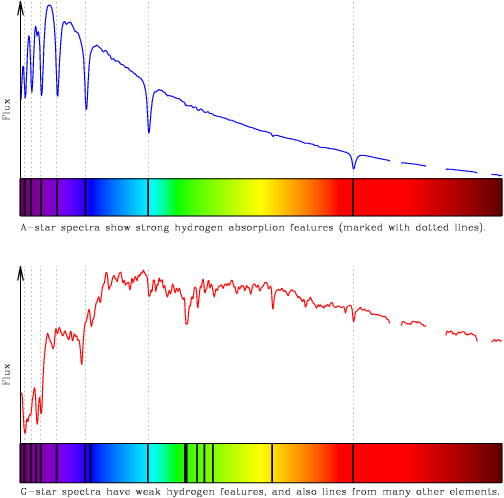
\includegraphics[width=0.9\textwidth,trim={0cm 9.75cm 0cm 0cm},clip]{Images/spectrum.png}
        \caption{The spectrum of a star.}
        \label{fig:stellar_spec}
    \end{subfigure}
    \hfill
    \begin{subfigure}[b]{0.75\textwidth}
        \centering
        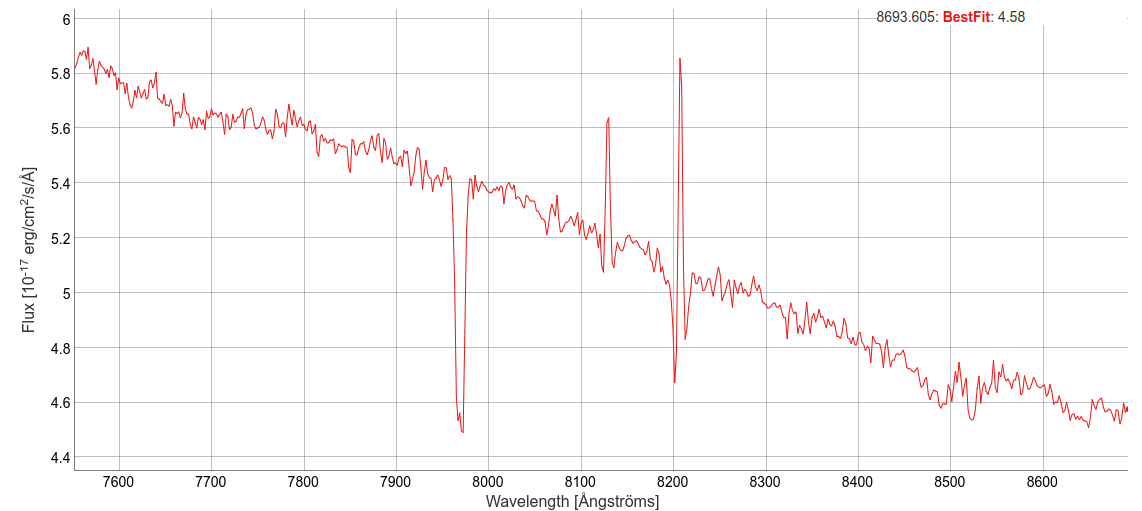
\includegraphics[width=0.9\textwidth,trim={0cm 0cm 0cm 1cm},clip]{Images/gal_spec.png}
        \caption{The spectrum of a galaxy.}
        \label{fig:gal_spec}
    \end{subfigure}
    \caption{}
    \label{fig:spec}
\end{figure}

\begin{enumerate}
    \setcounter{enumi}{11}
    \item \textit{[1 point]} The color bar below Figure \ref{fig:stellar_spec} (the stellar spectrum) is an alternative representation of the spectrum. How do the features in the Flux vs. Wavelength plot correspond to the features on the color bar?

    \item \textit{[3 points]} What differences do you notice between the stellar spectrum and the galaxy spectrum? What are some similarities? Hypothesize as to \emph{why} the spectrum of a star differs from that of a galaxy.
\end{enumerate}

\begin{figure}[h!]
    \centering
    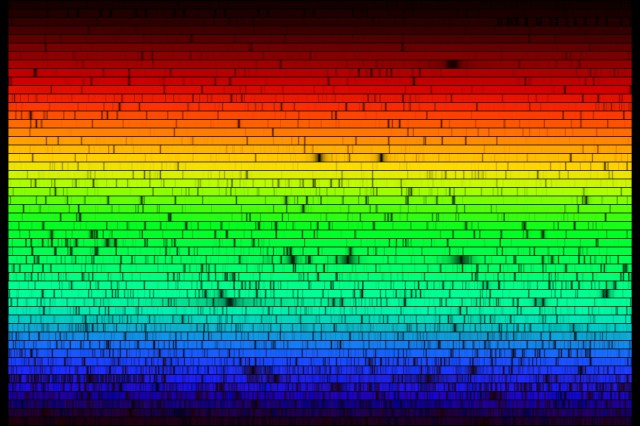
\includegraphics[width=0.7\textwidth]{Images/sun_spec.jpg}
    \caption{The spectrum of the Sun. Note that the actual spectrum should be one long, horizontal color gradient (like the ones seen through your diffraction gratings) -- this spectrum has been broken up into rows to fit onto the page and to show more detail.}
    \label{fig:sun}
\end{figure}

\noindent
Now, let's look at the spectrum of our Sun in Figure \ref{fig:sun}.

\begin{enumerate}
    \setcounter{enumi}{13}
    \item \textit{[1 point]} How is the Sun's spectrum different from the lamp spectra and the light bulb spectrum?
\end{enumerate}

Let's put everything we've seen in this lab together! Figure \ref{fig:types} shows three different types of spectra and how they're formed --- you have now seen all three today. Blackbodies emit across all wavelengths and thus have a \textbf{continuous spectrum} (the light bulb). A sample of gas is usually a conglomerate of multiple different chemical elements, so when the atoms of a gas are heated, they emit light at certain wavelengths, thus forming an \textbf{emission spectrum} (the lamps). By contrast, if light from a blackbody or a continuous spectrum passes \emph{through} a gas, the atoms of the gas absorb some light, yielding an \textbf{absorption spectrum} (the Sun). Due to the quantum nature of atoms, each element and molecule absorbs or emits at a unique set of wavelengths; each element has its own spectral ``fingerprint'' that can be used to uniquely identify the chemical makeup of an object.

\begin{figure}[h!]
    \centering
    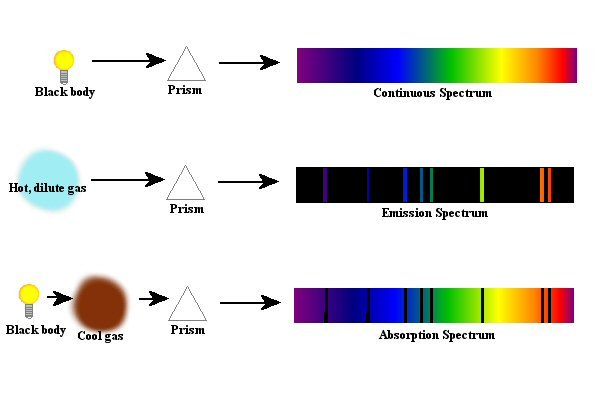
\includegraphics[width=0.9\textwidth,trim={0cm 2cm 0cm 1cm},clip]{Images/emission_v_absorption.jpg}
    \caption{Types of spectra.}
    \label{fig:types}
\end{figure}

\begin{enumerate}
    \setcounter{enumi}{14}
    
    \item \textit{[3 points]} Which type of spectrum matches the Sun's spectrum? The light bulb spectrum? The lamp spectra?


    \item \textit{[2 points]} Why does the Sun have that particular type, but not one of the other
    two? \\
    \textit{Hint: we observe light coming from the Sun's photosphere, but the
    Sun's corona lies between the photosphere and us...} 

\end{enumerate}

\subsection{Decomposing the Stars}
The spectral fingerprints we just explored allow astronomers to probe the chemical compositions of stars, galaxies, and planets. If we see an absorption line that we know is from carbon, then we know that there must be carbon in the star. The deeper the carbon absorption line in the spectrum, the more carbon there must be.

\medskip \noindent
Check Courseworks for the "Stellar Spectra Activity" document in the Lab 4 folder. This should be a PDF document with a few pages. Within this document, there are two real spectra from stars, labelled in orange, and some example spectra of seven specific elements (like the ones you just looked at with the lamps) labelled in blue. The stellar spectra has already been (roughly) lined up with each element for you. Each page has different elements on it that are lined up with the stellar spectra.


\begin{enumerate}
    \setcounter{enumi}{16}

    \item \textit{[2 points]} Go through the activity and list which elements you can see lines for
    in \textbf{Star 1}, then do the same for \textbf{Star 2}. 
    
    \item \textit{[2 points]} Which elements are found in \emph{both} stars? Which elements are only
    found in one star? 
\end{enumerate}

%\url{https://mrmacha.weebly.com/uploads/5/0/3/9/50390227/star_emission_spectrum_ws.pdf}

%%%%%%%%%%%%%%%%%%%%%%% REDSHIFT %%%%%%%%%%%%%%%%%%%%%%%
\section{Spectra and Motion: Oneshift, Twoshift, Redshift, Blueshift}
%Redshift and Blueshift

Spectra are not only useful for chemistry -- we can also use spectroscopy to study the \emph{motions} of astronomical bodies. Much like how the pitch of an ambulance changes as it moves towards or away from you, the wavelength of light changes depending on the motion of the light source -- this is a manifestation of the \emph{Doppler effect}. As a source of light moves towards you, the emitted light waves are \emph{compressed}, yielding shorter, bluer wavelengths: this is called \emph{blueshift}. Similarly, if a source of light is moving away from you, the light waves are \emph{stretched}, yielding longer, redder wavelengths: this is called \emph{redshift}. For fun, you can check out \url{https://javalab.org/en/doppler_effect_and_redshift_en/} to see blueshift and redshift in action.

\begin{figure}[h!]
    \centering
    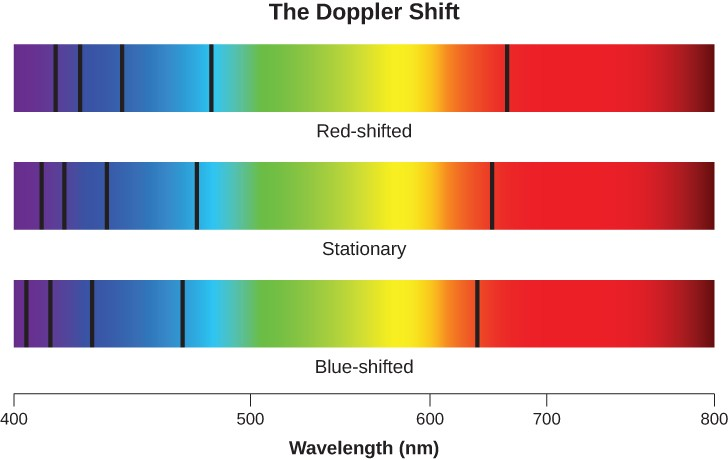
\includegraphics[width=0.75\textwidth]{Images/redshift.jpg}
    \caption{Redshift vs. Blueshift}
    \label{fig:redshift}
\end{figure}

\medskip \noindent
This redshift or blueshift manifests itself in the spectra of moving objects, as shown in Figure \ref{fig:redshift}. The middle row of Figure \ref{fig:redshift} shows the spectrum in the \emph{rest-frame} of the object -- that is, this is the spectrum we would observe if the object were perfectly stationary.

\begin{enumerate}
    \setcounter{enumi}{18}

    \item \textit{[3 points]} Look at the \textbf{top row} of Figure \ref{fig:redshift}, where the
    source is moving \emph{away}. Compared to the stationary spectrum in the
    middle, which way did the lines move, and are those wavelengths longer or
    shorter? What is this called?

    \item \textit{[3 points]} Now look at the \textbf{bottom row}, where the source is moving
    \emph{towards}. Which way did the lines move, and are those wavelengths longer or
    shorter? What is this called?

    \item \textit{[1 point]} Because the Universe is expanding, most objects are moving
    \emph{away} from us. So what should we expect to see in the spectrum of a
    typical galaxy, compared to its rest-frame spectrum?
\end{enumerate}

%%%%%%%%%%%%%%%%%%%%%%% REFLECTION %%%%%%%%%%%%%%%%%%%%%%%
\section{Reflection}

\begin{enumerate}
    \setcounter{enumi}{21}
\item \textit{[1 points]} Take a few minutes to reflect on your work today. What did you learn? Did
anything click, or connect to something you already knew from another
class, or from your own field? Did today's lab raise any questions? 
\end{enumerate}

\end{document}
